\documentclass[12pt]{article}
\usepackage{amsmath}
\usepackage{graphicx}
\usepackage{hyperref}
\usepackage[latin1]{inputenc}
\usepackage{enumitem}
\usepackage[margin=0.5in]{geometry}
\usepackage[LGRgreek]{mathastext}
\setlist[itemize]{noitemsep, topsep=0pt}
\title{12. Linear Regression}

\begin{document}

\begin{center} \textbf{Ch. 5 and 13: Linear Regressions}
\end{center}

\noindent \textbf{Part I:} (mostly review, hw 9)\\

In a regression analysis, we use independent variables/predictors (x) to try to predict the dependent variable/response (y). \\

From constructing a scatterplot, you can determine if there is a positive or negative relationship between the predictor and the response. \\

A negative slope means as the value in one variable increases, the value in the other decreases. If there is a positive slope, then as values in one variable increases, then the value in the other variable also increases.\\

We can summarize the relationship between the predictor and response with a linear regression model:\\
$$ Y = \alpha + \beta x + e $$

\begin{center}
    $\beta$ is the true slope, $\alpha$ is the true y-intercept, $e$ is the error term 
\end{center}

*Note that the Greek letters here still mean "true value", which means that we will have formulas to predict those parameters and do hypothesis testing!\\

\noindent \textbf{Assumptions:}
\begin{itemize}
\item $e_{i} \sim N(0,\sigma^{2})$
\item All $e_{i}$ are independent of one another\\
\end{itemize}

\noindent \textbf{Implications:}
\begin{itemize}
\item
$Y$ is a random variable that follows a normal distribution with $E(Y_{i})=\alpha + \beta x_{i}$ and $Var(Y_{i}) = \sigma^{2}$. 
\item
All of the $Y_{i}, Y_{j}$ are independent. 
\end{itemize}
\vspace{5mm}

\noindent With these assumptions, we have a way of predicting $\alpha$ and $\beta$ by a method of \textbf{``least squares"} and getting a predicted linear model: \\
$$\hat{y} = a + bx$$

*Note that this is $a$ and $b$, which are estimated values, whereas $\alpha$ and $\beta$ are the true parameters of the linear regression. And $\hat{y}$ is the predict response.\\

$b=\cfrac{\sum_{i}(x_{i}-\bar{x})(y_{i}-\bar{y})}{\sum_{i}(x_{i}-\bar{x})^{2}} = \cfrac{S_{xy}}{S_{xx}}$\\

$a = \bar{y}-b\bar{x}$ \\

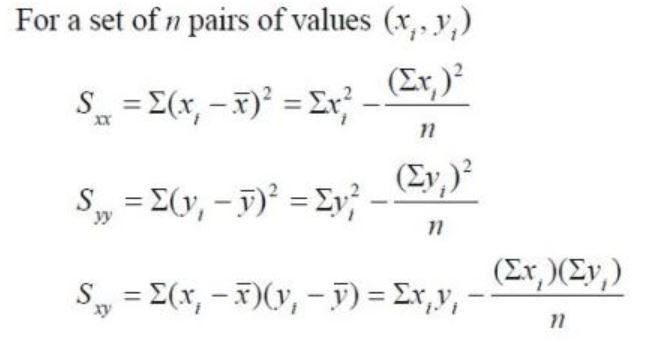
\includegraphics[scale = .75]{pic.JPG} \\

A residual ($\hat{e}_i$) is the difference between the true observed $y$ and the predicted value $\hat{y}$:\\
$$\hat{e}_i = y - \hat{y}$$

Recall the assumption that the error term is normally distributed with a mean of 0 and variance $\sigma^2$. We can find an estimate of this variance by finding the \textbf{mean square error} (MSE):\\
$$MSE = \cfrac{SSE}{n-1}$$

\noindent Sum of Squares Error (SSE) = $\sum_{i} (\hat{e}_i^{2}) = \sum_{i}(y_{i}-\hat{y}_i)^{2} $\\

\noindent Sum of Squares Regression (SSR) $ = \sum_{i}(\hat{y}_i-\bar{y})^{2} $\\

\noindent Sum of Squares Total (SST) $ = SSR + SSE = \sum_{i}(y_{i}-\bar{y})^{2}$\\

These values (along with some other relevant numbers) can be organized in an ANOVA table. \\

\noindent ANOVA Table: \\
\vspace{-5mm}
\begin{center}
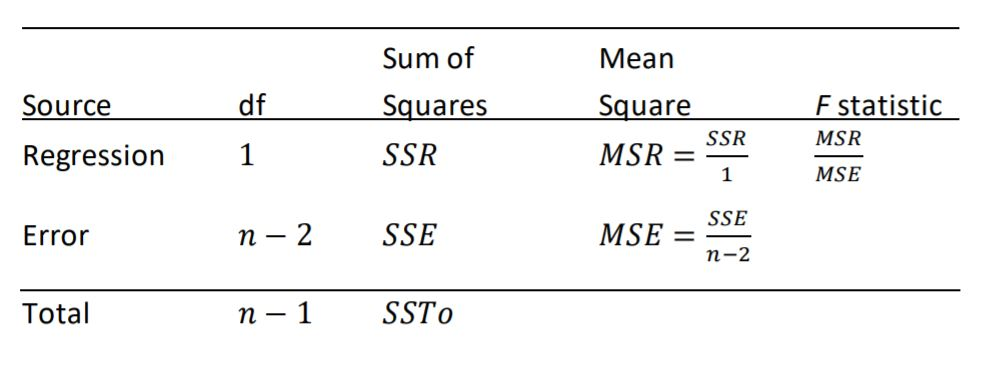
\includegraphics[scale=0.75]{ANOVAtable.JPG}
\end{center}

The standard error of residuals, denoted $s_{e}$ is equivalent to $\sqrt{MSE}$. Also, $\hat{\sigma}^2 = MSE$. \\

\noindent \textbf{Some examples} \\
\begin{enumerate}[noitemsep,topsep=0pt]
\item
Given three points: (1,3), (2, 4), (4, 6); calculate $S_{xx}$ and $S_{yy}$\\
\item
\noindent Fill in the blanks of the ANOVA table. \\

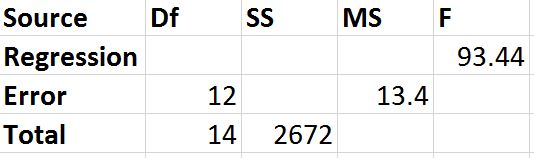
\includegraphics[]{blanktable.JPG}\\
%How many based on your answer to degrees of freedom for %regression, how many independent variables are in the model?
\item
\noindent Calculate $s_{e}$, which is the standard error of residuals.\\
\item
Calculate $\hat{\sigma}^{2}.$
\end{enumerate}
\vspace{5mm}
\noindent \textbf{Answers:}
\begin{enumerate}
\item
$s_{xx} = 14/3, s_{yy} = 14/3$
\item 
There's more than one approach to solve this problem, here's one way:\\
Degrees of freedom for regression is $14 - 12 = 2$, which is equal to the number of independent variables in a model. You've probably seen $df_R$ = 1, because there is only one predictor \\
$\cfrac{SSE}{df} = MSE$, so $SSE = MSE *df = 13.4*12 = 160.8$\\
Next, $SSR+SSE=SST$ by definition, so $SSR = SST-SSE = 2672 - 160.8 = 2511.2$\\
Since $MSR=SSR/df = 2511.2/2 = 1255.6$\\
Lastly, we can check that our answer is correct by calculating the F-stat with our numbers: $F=\cfrac{MSR}{MSE}=\cfrac{1255.6}{13.4} = 93.7$, which is close enough to the value in the table (93.44), small differences can be due to rounding. 


\item
$s_{e}=\sqrt{MSE}=\sqrt{13.4}=3.66$
\item
The predictor for variance is the MSE.\\
$\hat{\sigma}^{2} = MSE = 13.4$
\end{enumerate}

\noindent \textbf{Part II:} Inferences and residual analysis \\

First, we have \textbf{hypothesis testing}. Similar to previous chapters, follow the 5-steps:\\

(1) Null hypothesis: $H_0: \beta =0$\\

(2) Alternative: $H_1: \beta \neq 0$\\

(3) T-stat: $t_{obs} = \frac{b}{\sqrt{\frac{MSE}{S_{xx}}}}$\\
The denominator is the formula for $s_b$ (estimate of the standard error of the slope)\\

(4) Rejection region: find the critical value $t_{\alpha/2}$ that has $n-2$ degrees of freedom\\

(5) Decision: Reject $H_0$ if $|t_{obs}| > t_{\alpha/2}$\\

\textbf{Confidence interval}:
$$b \pm t_{\alpha/2}\sqrt{\frac{MSE}{S_{xx}}}$$

\textbf{Residual analysis:}\\

We can look at residuals to assess our original assumptions. Specifically a graph with the residuals on the y-axis and the predicted values on the x-axis. If we see no relationship, then our assumptions are likely true for the data. You don't want to see fanning either. \\

We can detect an outlier by looking at \textbf{leverage}.
$$h_{ii} = \frac{1}{n} + \frac{(x_i-\bar{x})^2}{S_{xx}}$$

Rule of thumb: High leverage if $h_{ii}$ is greater than \textbf{2 times} the average leverage, (average leverage = \textbf{(k+1)/n} , k = number of predictors, you will usually see in this class 2/n since k = 1.)\\

Or we can look at the \textbf{standardized residuals}.
$$r_i = \frac{\hat{e}_i}{\sqrt{MSE(1-h_{ii})}}$$

Rule of thumb: Outlier if $r_i > 2$ or $r_i < -2$. You may be asked to identify the outliers on a plot of standardized residuals. 
\end{document}